\documentclass[a4paper, 12pt]{article}

\usepackage[utf8]{inputenc}
\usepackage[russian]{babel}
\usepackage{graphicx}
\graphicspath{{pictures/}}
\DeclareGraphicsExtensions{.pdf,.png,.jpg}
\usepackage[unicode, pdftex]{hyperref}
\usepackage{color}
\usepackage{float}
\setlength{\parindent}{5ex}
\setlength{\parskip}{1em}
\usepackage{indentfirst}

\begin{document}

\begin{titlepage}
  \centerline {Санкт-Петербургский политехнический университет}
  \centerline { им. Петра Великого}
  \centerline { }
  \centerline {Институт прикладной математики и механики} 
  \centerline {Кафедра "Прикладная математика"}
  \vfill
  \centerline{\textbf{Отчёт}}
  \centerline{\textbf{по лабораторной работе №8}}
  \centerline{\textbf{по дисциплине}}
  \centerline{\textbf{"Математическая статистика"}}
  \vfill
  \hfill
  \begin{minipage}{0.45\textwidth}
  Выполнил студент:\\
  Дроздова Дарья Александровна\\
  группа: 3630102/80401 \\
  \\
  Проверил:\\
  к.ф.-м.н., доцент \\
  Баженов Александр Николаевич
  \end{minipage}
  \vfill
  \centerline {Санкт-Петербург}   
  \centerline {2021 г.}  
\end{titlepage}

\newpage
\setcounter{page}{2}
\tableofcontents

\newpage
\listoffigures

\newpage
\listoftables

\newpage
\section{Постановка задачи}

Провести дисперсионный анализ с применением критерия Фишера по данным регистраторов для одного сигнала. Определить области однородности сигнала, переходные области, шум / фон.

Длину сигнала принять $1024$

\newpage
\section{Теория}

Анализ проводится по следующему алгоритму:
\begin{enumerate}
	\item Строим гистограмму значений, в которой столбы отвечают за следующие области:
	\begin{itemize}
		\item Столбец с наибольшим значением - фон
		\item Столбцы с малыми значениями - переходы
		\item Второй по величине столбец после фона - сигнал
	\end{itemize}
	\item Устранение явных выбросов с помощью медианного фильтра.
	\item Разделение сигнала на области: сигнал, фон, переход.
	\item Разделение областей на типы по критерию Фишера.
\end{enumerate}

\subsection{Внутригрупповая дисперсия}

Внутригрупповая дисперсия $s^2_{intaGroup}$ вычисляется по следующей формуле
\begin{equation}
	s^2_{intaGroup} = \frac{1}{k}\sum^k_{i=1}s_i^2 = \frac{1}{k}\sum^k_{i=1} \frac{\sum^n_{j=1} (x_{ij} - X_{\mbox{ср}})^2}{k-1}
\label{eq:1}
\end{equation}
где $X_{\mbox{ср}}$ - среднее для части выборки, $k$ - количество частей выборки.

Внутригрупповая дисперсия является дисперсией совокупности и рассматривается как среднее значение выборочных дисперсий.

\subsection{Межгрупповая дисперсия}

Межгрупповая дисперсия $s^2_{interGroup}$ вычисляется по формуле
\begin{equation}
	s^2_{interGroup} = k \frac{\sum^k_{i=1}(X_{i_{\mbox{ср}}} - X_{\mbox{ср}})^2}{k-1}
\label{eq:2}
\end{equation}
где $X_{1_{\mbox{ср}}}, X_{2_{\mbox{ср}}},...,X_{k_{\mbox{ср}}}$ - среднее значение для подвыборок, $X_{\mbox{ср}}$ - среднее значение этих средних значений подвыборок.

\subsection{Критерий Фишера}

Значение Критерия Фишера определяется формулой
\begin{equation}
	F = \frac{s^2_{interGroup}}{s^2_{intaGroup}}
	\label{eq:3}
\end{equation}

\newpage
\section{Реализация}

Лабораторная работа выполнена на языке программирования Python в среде разработки PyCharm. С использованием библиотек numpy и skipy.

Код программы расположен в репозитории GitHub по ссылке: \url{}

\newpage
\section{Результаты}

\begin{figure}[H]
\center{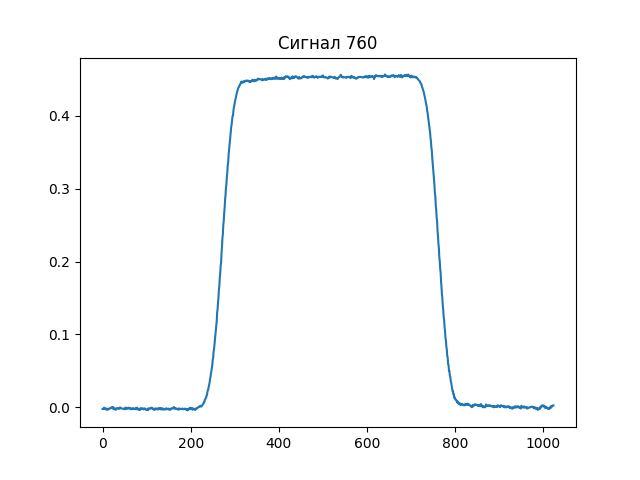
\includegraphics[scale=0.6]{Figure_1}}
\caption{Входной сигнал}
\end{figure}

\begin{figure}[H]
\center{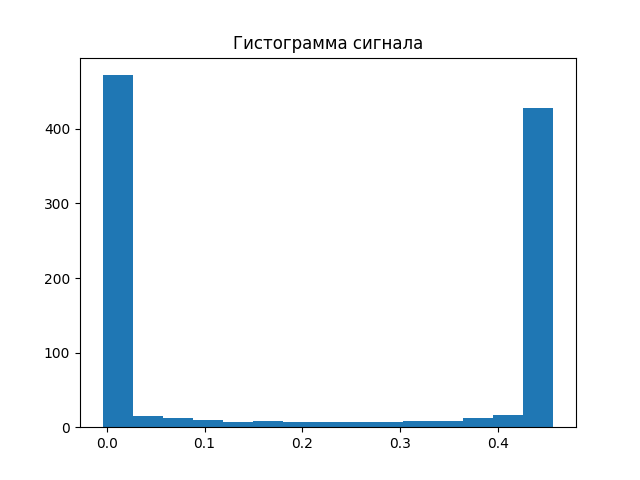
\includegraphics[scale=0.6]{Figure_2}}
\caption{Гистограмма сигнала}
\end{figure}

\begin{figure}[H]
\center{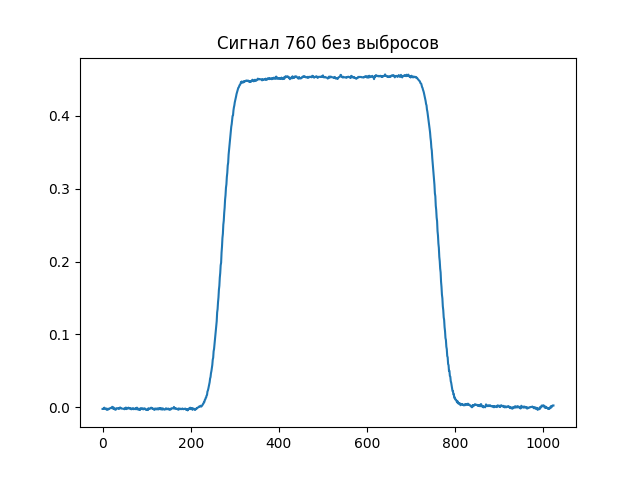
\includegraphics[scale=0.6]{Figure_3}}
\caption{Сигнал без выбросов}
\end{figure}

\begin{figure}[H]
\center{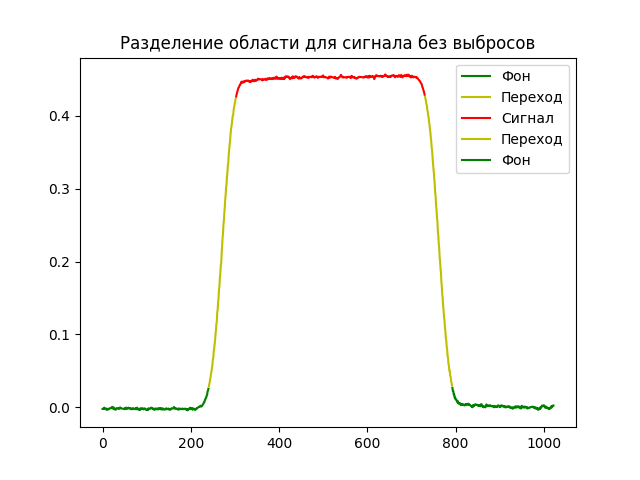
\includegraphics[scale=0.6]{Figure_4}}
\caption{Разделение областей для данных сигнала с устранением выбросов}
\end{figure}


\begin{table}[H]
\begin{flushleft}
\begin{tabular}{|c|c|c|c|c|c|}
\hline 
Промежуток & Тип & Кол-во разбиений & $s^2_{intarGroup}$ (\ref{eq:1}) & $s^2_{interGroup}$( \ref{eq:2}) & $F$ (\ref{eq:3}) \\ 
\hline 
1 & Фон & 11 & 0.000016 & 0.000142 & 8.863024 \\ 
\hline 
2 & Переход & 31 & 0.000001 & 0.552984 & 430130.786850 \\ 
\hline 
3 & Сигнал & 4 & 0.000437 & 0.000002 & 0.049010 \\ 
\hline 
4 & Переход & 31 & 0.000001 & 0.553874 & 397759.690521 \\ 
\hline 
5 & Фон & 5 & 0.000093 & 0.000041 & 0.440380 \\ 
\hline 
\end{tabular}

\caption{Характеристики выделенных областей}
\end{flushleft}
\end{table}


\newpage
\section{Обсуждение}

Для входных данных сигнала были получены следующие области однородности: фон и сигнал, эти области однородны, так как значения критерия Фишера находятся вблизи 1.

На переходах значения критерия Фишера много больше 1, значит эти области неоднородны.
\end{document}
